\documentclass[12pt,a4paper,oneside]{article}

\usepackage[english]{babel}
\usepackage[T1]{fontenc}
\usepackage{multicol}
\usepackage[a4paper,top=20mm,left=30mm,right=15mm,bottom=15mm]{geometry}
\usepackage[monochrome]{color}
\usepackage{fontspec}
\usepackage{tocloft}
\usepackage[nottoc,numbib]{tocbibind}
\usepackage{fancybox} 
\usepackage{setspace}
\usepackage{ccicons}
\usepackage{anyfontsize}
\usepackage{lipsum}
\usepackage{indentfirst}
\usepackage{soul}
\usepackage[hidelinks]{hyperref}
\usepackage{mathtools}   
\usepackage{tikz}
\usepackage{csquotes}
\usepackage{wrapfig}
\usepackage{background}
\usepackage{longtable}
\usepackage[acronym]{glossaries}
\usetikzlibrary{calc}
\usepackage{float}
\usepackage[
    backend=biber,
    style=ieee,
]{biblatex}
\addbibresource{manufacturing.bib}
\usepackage{afterpage}
\newcommand\blankpage{%
    \null
    \thispagestyle{empty}%
    \addtocounter{page}{-1}%
    \newpage}
\setmainfont[Ligatures=TeX]{Times New Roman}
\renewcommand{\cftsecleader}{\cftdotfill{\cftdotsep}}


\backgroundsetup{
    color=black,
    scale=1,
    opacity=1,
    angle=0,
    contents={
        \begin{tikzpicture}
            \draw [line width=0.75pt] ($ (current page.north west) + (2.5cm,-1cm) $) rectangle ($ (current page.south east) + (-1cm,1cm) $);
            \draw [line width=0.00pt] ($ (current page.north west) + (0.1cm,0.1cm) $) rectangle    ($ (current page.south east) + (0.1cm,0.1cm) $); 
        \end{tikzpicture}
    }
}


\begin{document}

\begin{titlepage}

\begin{flushright}
%\textbf{\uppercase{\fontsize{12}{18} \selectfont {Group No: E2}}}
\end{flushright}


\center % Center everything on the page
{\setstretch{1.2}

\includegraphics[width=2in,keepaspectratio]{logo.png}\\[0.5cm]
\fontsize{16pt}{24}\selectfont \textbf{Project Report}\\[0.5cm]
\fontsize{16pt}{24}\selectfont \textbf{EGT 41206}\\[0.75cm]
\fontsize{24pt}{30}\selectfont \textbf{\uppercase{Whiteboard Eraser}}\\[1.5cm]
\fontsize{16pt}{24}\selectfont \textbf{By}\\[0.5cm]
\fontsize{12pt}{12}\selectfont {
}
\vspace{5cm}
\fontsize{12pt}{12}\selectfont \textbf { Gnanakeethan Balasubramaniam \\ EGT/16/00037}\\[0.5cm]


\vspace*{\fill}
\fontsize{12pt}{12}\selectfont \textbf {Department of Engineering Technology \\ Faculty of Technology\\University of Sri Jayewardenepura\\ Sri Lanka}\\[0.5cm]
}

\vfill % Fill the rest of the page with whitespace

\end{titlepage}


\pagenumbering{roman}

\newpage
\tableofcontents

\listoffigures
\newpage
\pagenumbering{arabic}
\setcounter{page}{1}


\section{Introduction}

A whiteboard eraser is usually used in many places. It is available in many sizes as well. It usually consists of two parts namely, a plastic grip and a soft area for cleaning. However some erasers have magnetic plates built into the surface below the soft area. The magnetic plates allow the erasers to hung on whiteboards made of iron compositions. 

These whiteboard erasers’ plastic grip are usually manufactured using Plastic moulding. The soft-core is made by cutting a solidified soft-rubber foam or a soft cloth material. The magnetic plate is usually made of iron compositions. 



\newpage
\section{Plasic grip}

The plastic grip is usually made using plastic moulding process. The process involves the following steps. 

\begin{enumerate}
    \item Fabrication of mould for testing
    \item Production Test
    \item Refining the mould designs
    \item Creating of die for mass production.
    \item Production of the part
\end{enumerate}


\subsection{Fabrication of Mould for testing}

The mould design would be usually made out of hard materials. The moulds for the process of plastic injection moulding is usually manufactured using CNC Machines (Electric Discharge Machining, Lathe, Milling). Typically these are made using hardened steel, pre-hardened steel, aluminium, and/or beryllium-copper alloy.

\subsection{Production Test}

In this process the injection mould is tested by creating a small set of production grade Plastic grips. Eventhough it may seem unnecessary to manufacture and test, due to the large cost associated with this step. It will be cost-effective than manufacturing a faulty product.

\subsection{Mould Design Refinement}

The mould is redefined with feedback from the initially manufactured test products. The process repeats the production test until desired quality is achieved.

\subsection{Mould for mass production}

A new mould is then created for mass production using the design elements achieved earlier. The mould manufacturing process is same as previous, however the materials are changed to more durable ones. Thus hardened steel is a viable material for mould making. 
\cite{2018:Injection}


\subsection{Production of the part}

The part is then mass produced using industrial injection moulding machines.Usually the machines are capable of operating at speeds of manufacturing multiple parts at the same time.  

\begin{figure}[H]
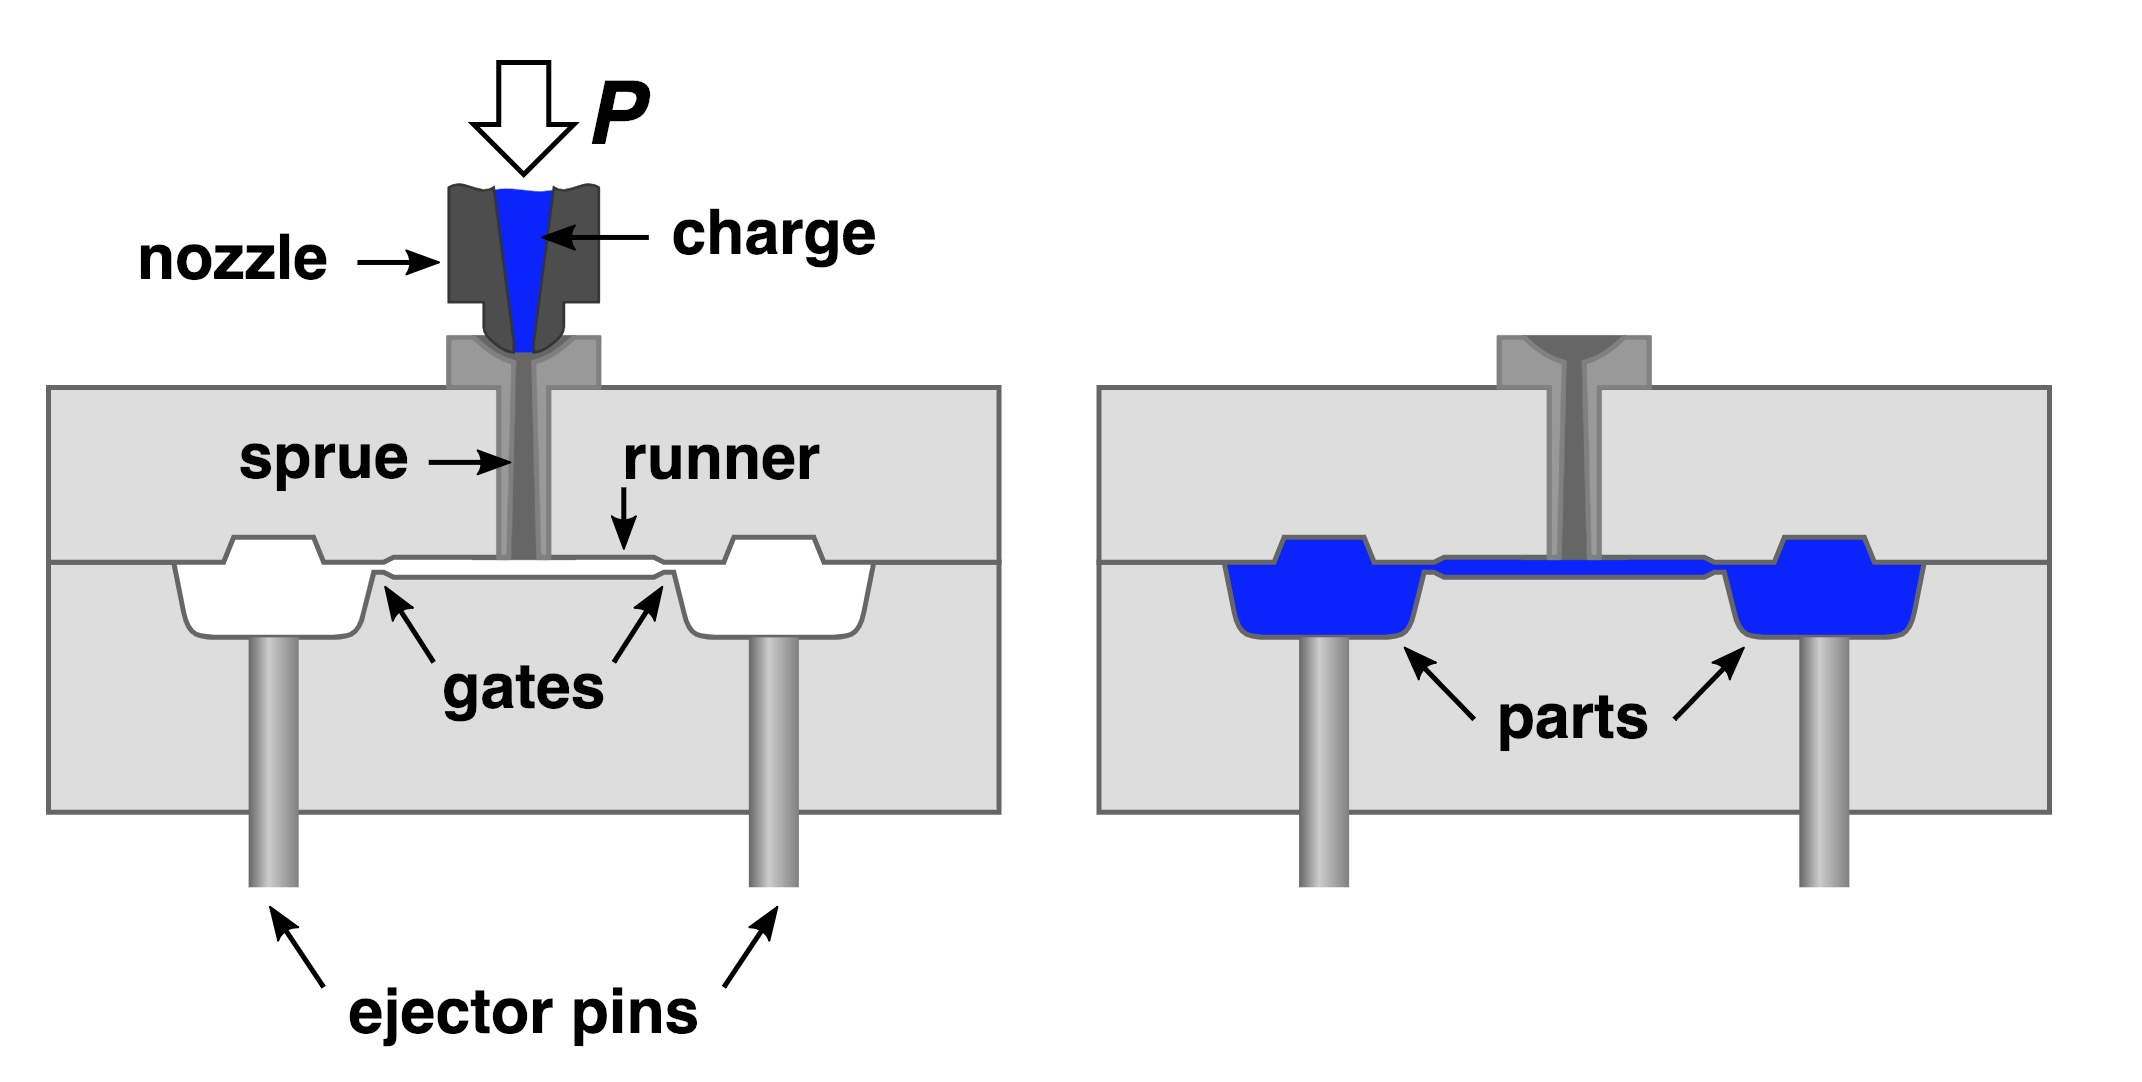
\includegraphics[width=0.5\textwidth]{injection-moulding}
\caption{Injection Moulding Process\cite{2018:InjectionImage}}
\end{figure}


\newpage

\section{Manufacturing of Rubber Core}

The rubber core is generally manufactured using a soft-rubber foam. For that purpose, such rubber foam sheets are taken and cut into proper sheets. The Softcloth is then affixed on top using a permanent adhesive or temporary adhesive. 

\subsection{Procurement of Rubber Sheets}

These rubber sheets are manufactured in factories. They are usually available at generous sizes. We can choose a size ranging upwards from 6ftx3ft. These rubber sheets are formed by solidified rubber foams. They have properties to content excessive liquids. 

\begin{figure}[h]
    \centering
    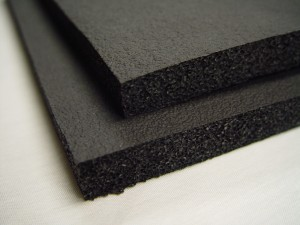
\includegraphics[width=0.5\textwidth]{rubber-foam}
    \caption{Rubber Foam Sheets}
\end{figure}



\subsection{Creation of Cutting Steel}

In order to cut rubber sheets, we need to create steel cutting shapes. For this purpose, It is better to use Electric Discharge Machining to create the cut steel

\subsection{Production of Rubber Core}

The produced die is punched through the Rubber sheet to produce the Rubber cores. The rate of production in this section will be depending on the die-cuts per punch. A punch usually takes about a second. Generally we can manufacture 20 of these die-cut Rubber cores. 

\subsection{Procurement of Soft Cloth}

Soft cloth is necessary to be placed on top of the rubber core to facilitate a even smoother operation. The soft cloth can be obtained from a textile manufacturing plant and it can be made to custom specifications, such as thickness, special materials. The cloth is usually made out of very soft fibres to add softness.


\subsection{Fitting of Soft Cloth}

The soft cloth can be fixed using two mechanisms. Namely Velcro mechanism and Permanent adhesive. In these methods, it is better to use Velcro mechanism for longevity of the product. In that sense, we procure velcro-sheets cut as per our requirements, and permanently paste the opposites onto the rubber-core and the soft-cloth. Thereafter it will be easier for the customers to replace the softcloth. 

However the velcro must allow seeping of the liquids through itself in order to provide a smooth experience to the user.


\newpage

\section{Assembly of Rubber Core and Magnetized Sheet}

\subsection{Procurement of Magnetized Steel Sheet Cuts}
The magnetized steel sheets can be obtained in the market as per our specifications and as per the shape needed. These sheets must have a limited magnetic ability, so as not to interfere with the other materials. 

\subsection{Application of Adhesive Material}
The magnetic sheet is coated with adhesive and the rubber core is thereafter pressed onto it with a high pressure. Thus it attaches both the parts firmly. The strength of the adhesiveness depends on the material used as adhesive. 


\newpage

\section{Final Assembly}
Thereafter the final assembly is done between the components completed before.
\begin{itemize}
    \item Plastic Grip (Cavity)
    \item Rubber Core and Magnetic Sheet
\end{itemize}

\subsection{Fixation of Parts}

Adhesive material is then applied on the inside of the plastic cavity where the plastic cavity and the rubber core meet. Usually to the inner-sidewalls of a whiteboard eraser. The fixing of parts is done by forcing the soft-rubber core into the plastic cavity. 


\begin{figure}[h]
    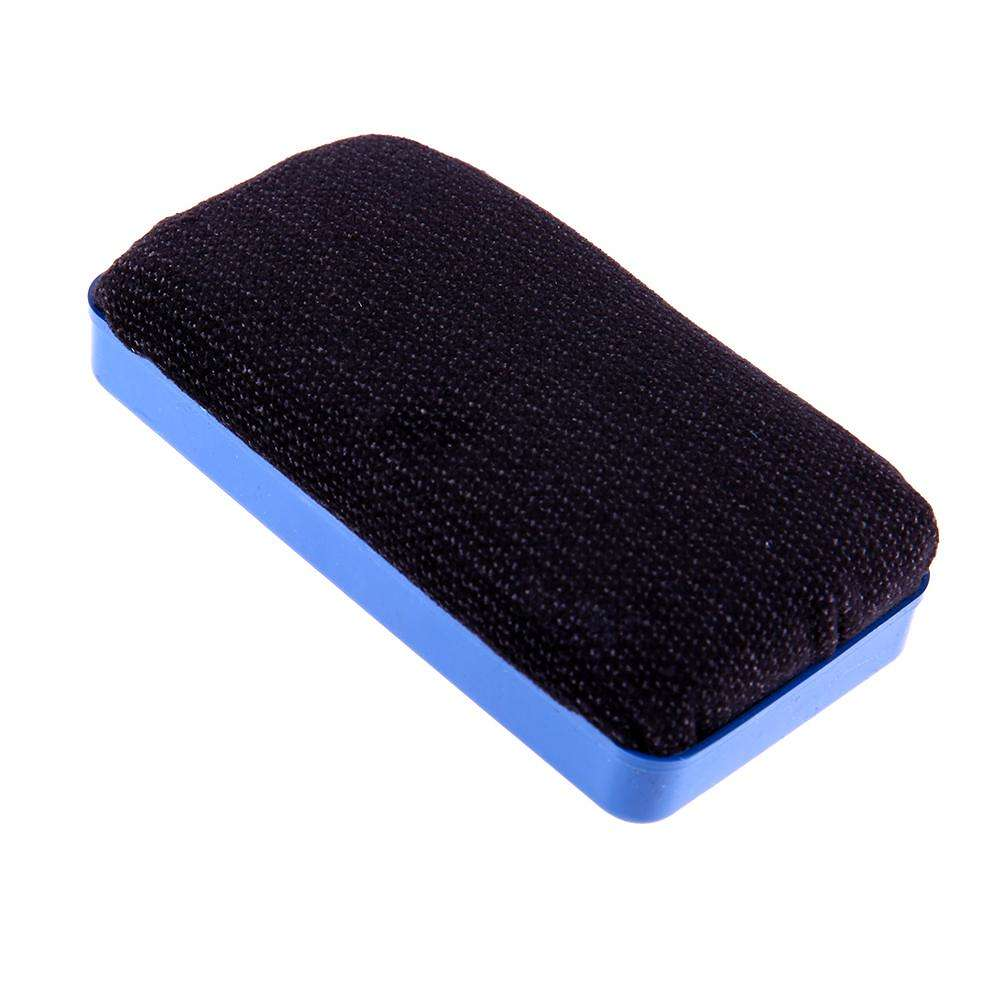
\includegraphics[width=1\textwidth]{whiteboard-magnetic}
    \caption{Magnetic Whiteboard Eraser.}
\end{figure}
\newpage

\clearpage
\addcontentsline{toc}{section}{References}
\printbibliography
\afterpage{\blankpage}

\end{document}
